In this section we discuss how to create a geometry file (\texttt{.geo}), with the geometry file being interpreted by \texttt{Netgen}~\cite{netgen} (the meshing tool in \texttt{NGSolve}) we first explain how to create shapes and geometries using a \texttt{.geo} file. \\
\\
Due to \texttt{Netgen} being the underlying interpreter of the \texttt{.geo} file we direct the user to the relevant Constructive Solid Geometry (CSG) documentation available at \href{http://netgen-mesher.sourceforge.net/docs/ng4.pdf}{\texttt{http://netgen-mesher.sourceforge.net/do\\cs/ng4.pdf}}. With this knowledge of this,  we next discuss how the requirements outlined in Section \ref{sectCalculatingMPT}, relating to the  domain $\Omega $, which contains the object $B$, can be specified.
 Finally we explain how to define material properties of the objects being simulated.
\subsection{Truncating the domain}\label{sectTruncating}
Since it is impossible to simulate an infinite computational domain we are required to create a truncated domain $\Omega$ whose boundary $\partial\Omega$ is sufficiently far from the object $B$. In order to do this in the \texttt{.geo} file we simply define a  region which is much larger than the object and place the object at its centre. An example of this is  presented in the \texttt{.geo} file  shown in Figure \ref{fig:ExampleSphere} along with a visualisation of the of the geometry obtained in \texttt{Netgen}.

\begin{figure}[H]
$$\begin{array}{cc}
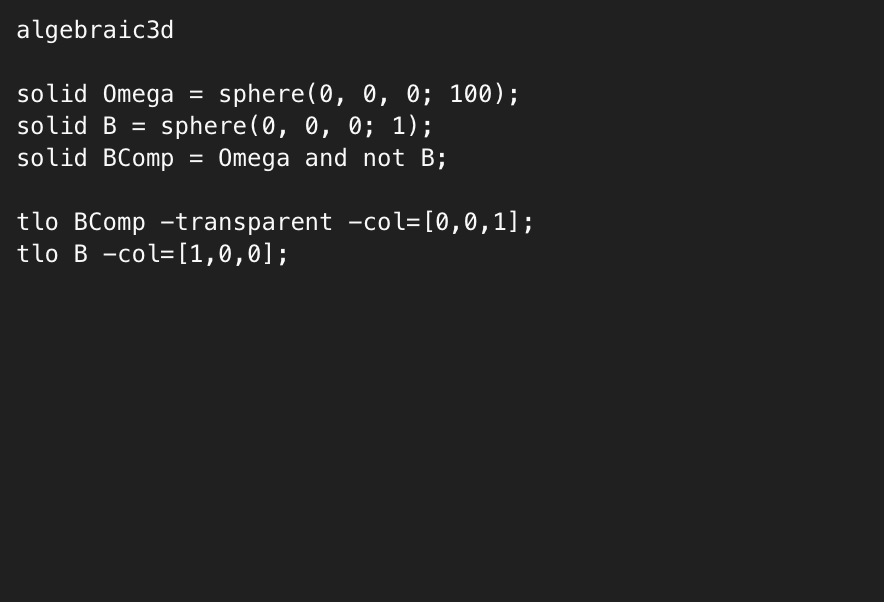
\includegraphics[width=0.48\textwidth, keepaspectratio]{Figures/ExampleSphere.png} & 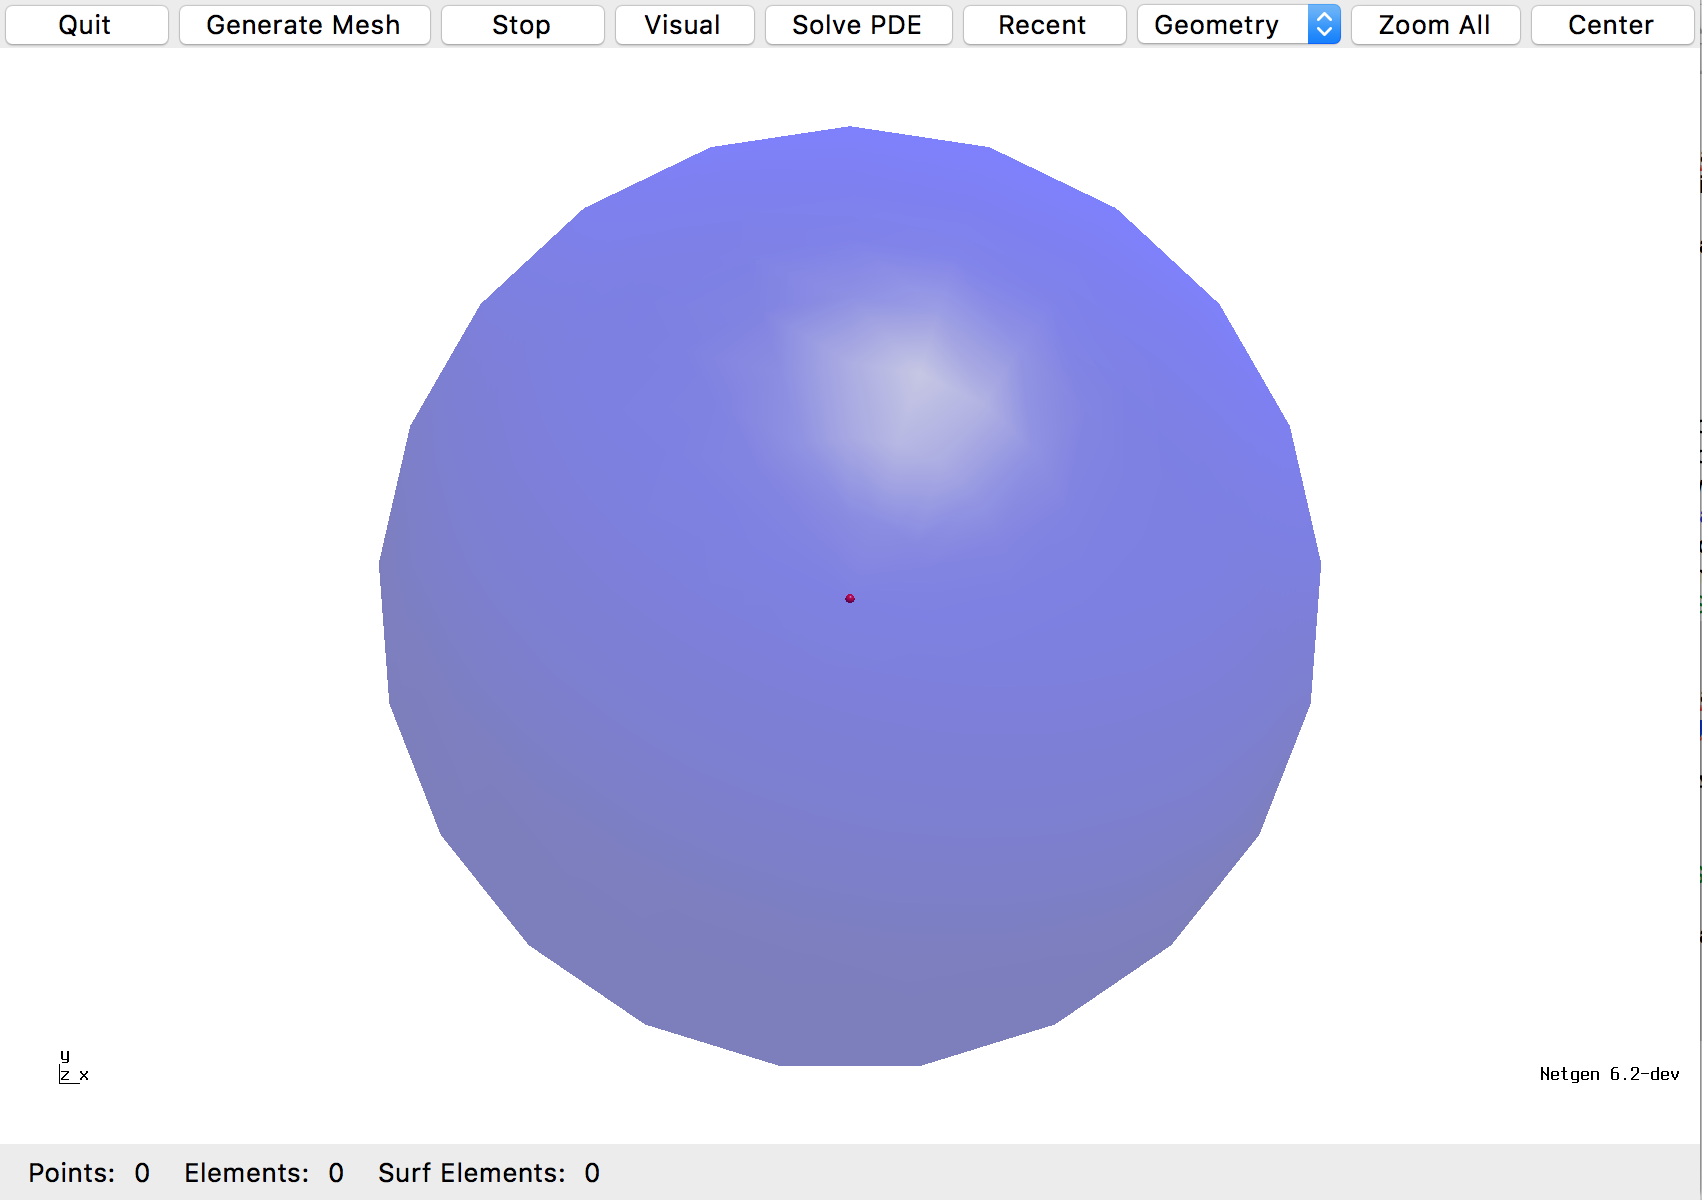
\includegraphics[width=0.48\textwidth, keepaspectratio]{Figures/ExampleSphereNetgen.png}\\
\textrm{\footnotesize{(a) Example of a \texttt{.geo} file describing a sphere in a sphere}} & \textrm{\footnotesize{(b) Visulisation of the \texttt{.geo} file in (a)}}
\end{array}$$
%\begin{figure}\label{LogvsLin}
\caption{Example of a \texttt{.geo} file (a) describing a sphere of unit radius contained in a domain consisting of a sphere with a radius of 100, with (b) a visualisation of of the constructed geometry using negten.}
\label{fig:ExampleSphere}
\end{figure}
\noindent
This example defines a unit sphere $B$ contained in a domain $\Omega$, which consists of a sphere with a radius of 100. Truncating the domain at a distance approximately 100 times the object size is sufficient for most cases. Next we discuss how to define the material properties of the different regions in the domain.
\subsection{Defining material properties}
To set the material parameters, the user is required to  label each region defined as a Top Level Object (tlo).  This is done by inserting a \texttt{\#} after each toplevel object followed by a label for the material, it's relative permeability $\mu_r$ and it's conductivity $\sigma_*$. We define the material properties for the example presented in the Section \ref{sectTruncating} in  the Figure \ref{fig:ExampleSphereMaterials}.

\begin{figure}[H]
\begin{center}
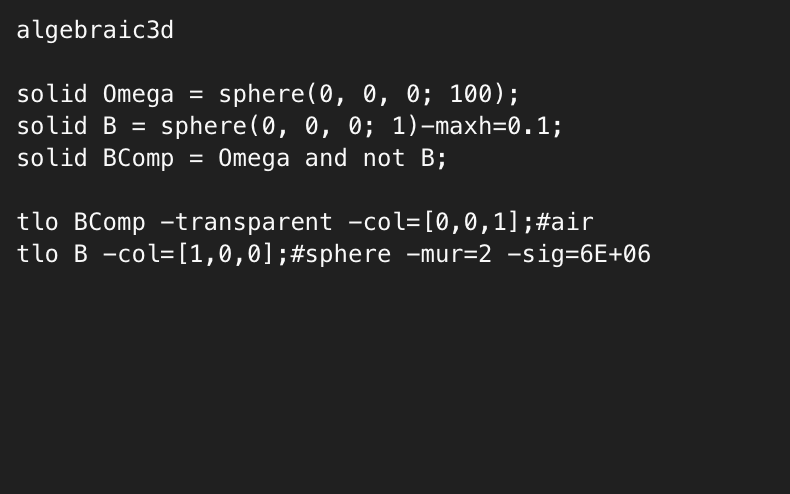
\includegraphics[width=0.5\textwidth]{Figures/ExampleSphereMaterials.png}
\caption{Image displaying an example of a \texttt{.geo} file with material properties defined for it's regions.}\label{fig:ExampleSphereMaterials}
\end{center}
\end{figure}
\noindent
In Figure \ref{fig:ExampleSphereMaterials}, \texttt{\#sphere -mur=2 -sig=6e+06} labels the object $B$ as \texttt{"sphere"} and defines it's material properties to be $\mu_r=2$ and $\sigma_*=6\times10^6 \text{S/m}$. The inclusion of \texttt{\#air} labels the non conducting region as \texttt{"air"}, which is a protected material and, therefore, does not require the user to input a value for $\mu_r$ or $\sigma_*$. Lastly,  note the inclusion of \texttt{-maxh=0.1} when defining the geometry of $B$. This is an inbuilt function of \texttt{Netgen} for meshing purposes allowing the user to specify a maximum element size for each region in the domain. This is useful since it allows the user to refine the mesh in the conducting region of the domain.\\
\\
Next, we specify the restrictions of the syntax for defining material properties. Any line which starts with \texttt{tlo} (which must have no spaces before) must also contain a material label defined as \texttt{\#material}. On the same line, the user must define both $\mu_r$ and $\sigma_*$ (unless the material is defined to be \texttt{\#air}), to do this the user must provide the flag \texttt{-mur=***} and \texttt{-sig=***} with at least one space between the two flags, but no spaces before or either of the equal signs, and with \texttt{***} replaced with value of the parameter. Note that  $\sigma_*$ should be specified in $\text{S/m}$. Some examples of this can be seen below, first the following examples are accepted,
\begin{align*}
&\texttt{tlo B -col=[1,0,0];\#sphere -mur=2 -sig=6E+06}\\
&\texttt{tlo B -col=[1,0,0];    $\quad$       \#sphere-mur=2 -sig=6E+06}\\
&\texttt{tlo B -col=[1,0,0];\#sphere   $\quad$    -mur=2   $\quad$  -sig=6E+06}
\end{align*}
However, the following examples will not work
\begin{align*}
&\texttt{tlo B -col=[1,0,0];\#sphere -mur = 2 -sig = 6E+06}\\
&\texttt{  tlo B -col=[1,0,0];\#sphere-mur=2 -sig=6E+06}\\
&\texttt{tlo B -col=[1,0,0];\#sphere -mur=2-sig=6E+06}\\
&\texttt{tlo B -col=[1,0,0];\#sphere}\\
&\texttt{-mur=2-sig=6E+06}
\end{align*}
Due to there being a space before or after the equal signs in the first; to a space before the \texttt{tlo} in the second; to the lack of a space between the definition of \texttt{-mur} and \texttt{-sig} in the third and due to the split two lines in the last.
\\
\\
We next consider the case of an object made up of multiple conducting regions follow the examples in Ledger, Lionheart and Amad~\cite{LedgerLionheartamad2019}. We define a conducting rectangular bar, $B$ which is a $2\times1\times1$ block made up 2 distinct sections, contained in a domain bounded by a sphere with radius of 100, as defined in the \texttt{.geo} file shown in Figure \ref{fig:DualBarExample}. Note that $B$ does not have units, the object $\alpha B$ has units with $\alpha$ being the size parameter specified in $\text{m}$ and $\alpha$ is specified later.

\begin{figure}[H]
\begin{center}
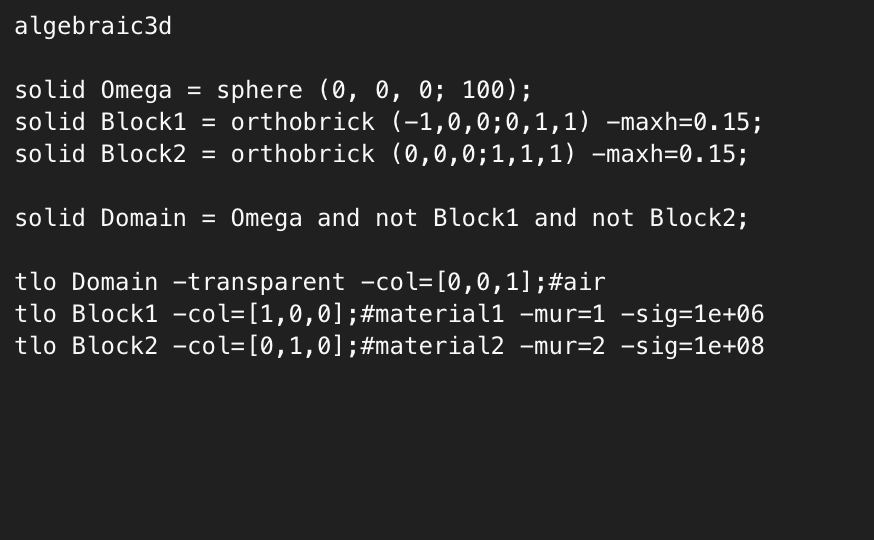
\includegraphics[width=0.5\textwidth]{Figures/DualBarExample.png}
\caption{Image displaying an example of a \texttt{.geo} file which defines a bar constructed of 2 regions with different material properties contained in a domain consisting of a sphere with a radius of 100.}\label{fig:DualBarExample}
\end{center}
\end{figure}
\noindent
In Figure \ref{fig:DualBarExample} we have defined two distinct regions \texttt{Block1} and \texttt{Block2} with materials \texttt{"Material1"} and \texttt{"Material2"} having different material properties, respectively.\\
\\
We finish this section with an example of two unit spheres which are constructed using the same material. An example of the \texttt{.geo} file can be seen in Figure \ref{fig:TwoSpheresExample}.

\begin{figure}[H]
\begin{center}
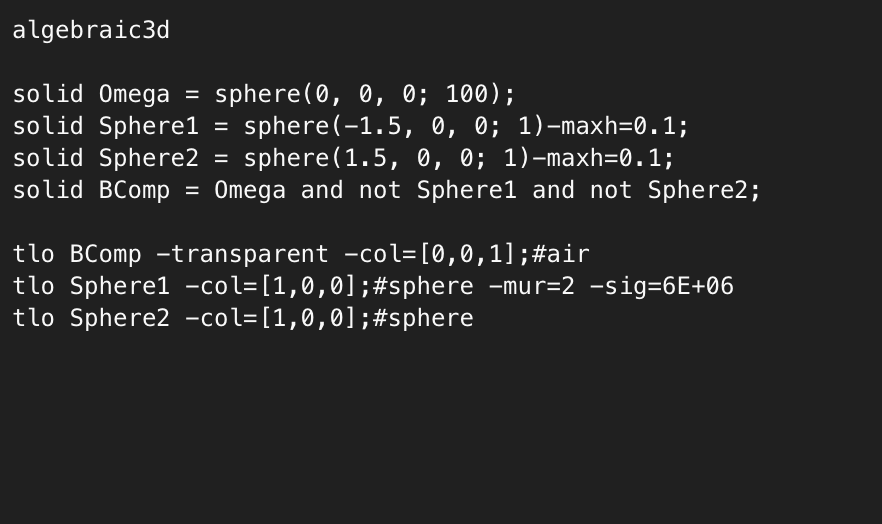
\includegraphics[width=0.5\textwidth]{Figures/TwoSpheresExample.png}
\caption{Image displaying an example of a \texttt{.geo} file which defines a bar constructed of 2 regions with different material properties contained in a domain consisting of a sphere with a radius of 100.}\label{fig:TwoSpheresExample}
\end{center}
\end{figure}
\noindent
This example demonstrates how we only need to define the material properties for \texttt{\#sphere} once even though there are two regions to which it will be applied. This makes it easier to change material properties for a whole geometry when made up of multiple \texttt{tlo}s. We expect this to be useful when working with more complex geometries such as that in the case of a rifle shell, which will be presented in Section \ref{sectRifle}. In the next Section we work through some specific examples.















